\begin{figure}[htb]
\centering
\includegraphics[page=4,width=0.33\textwidth]{\FCNCFigures/xTFW/showFake/NOMINAL/reg2mtau1b2jos_vetobtagwp70_highmet/BDTG_test.pdf}
\put(-30, 80){\textbf{(a1)}}
\includegraphics[page=5,width=0.33\textwidth]{\FCNCFigures/xTFW/showFake/NOMINAL/reg2mtau1b2jos_vetobtagwp70_highmet/BDTG_test.pdf}
\put(-30, 80){\textbf{(a2)}}
\includegraphics[width=0.33\textwidth]{\FCNCFigures/xTFW/BDT/roc_reg2mtau1b2jos.pdf}
\put(-70, 70){\textbf{(a3)}}\\
\includegraphics[page=4,width=0.33\textwidth]{\FCNCFigures/xTFW/showFake/NOMINAL/reg2mtau1b3jos_vetobtagwp70_highmet/BDTG_test.pdf}
\put(-30, 80){\textbf{(b1)}}
\includegraphics[page=5,width=0.33\textwidth]{\FCNCFigures/xTFW/showFake/NOMINAL/reg2mtau1b3jos_vetobtagwp70_highmet/BDTG_test.pdf}
\put(-30, 80){\textbf{(b2)}}
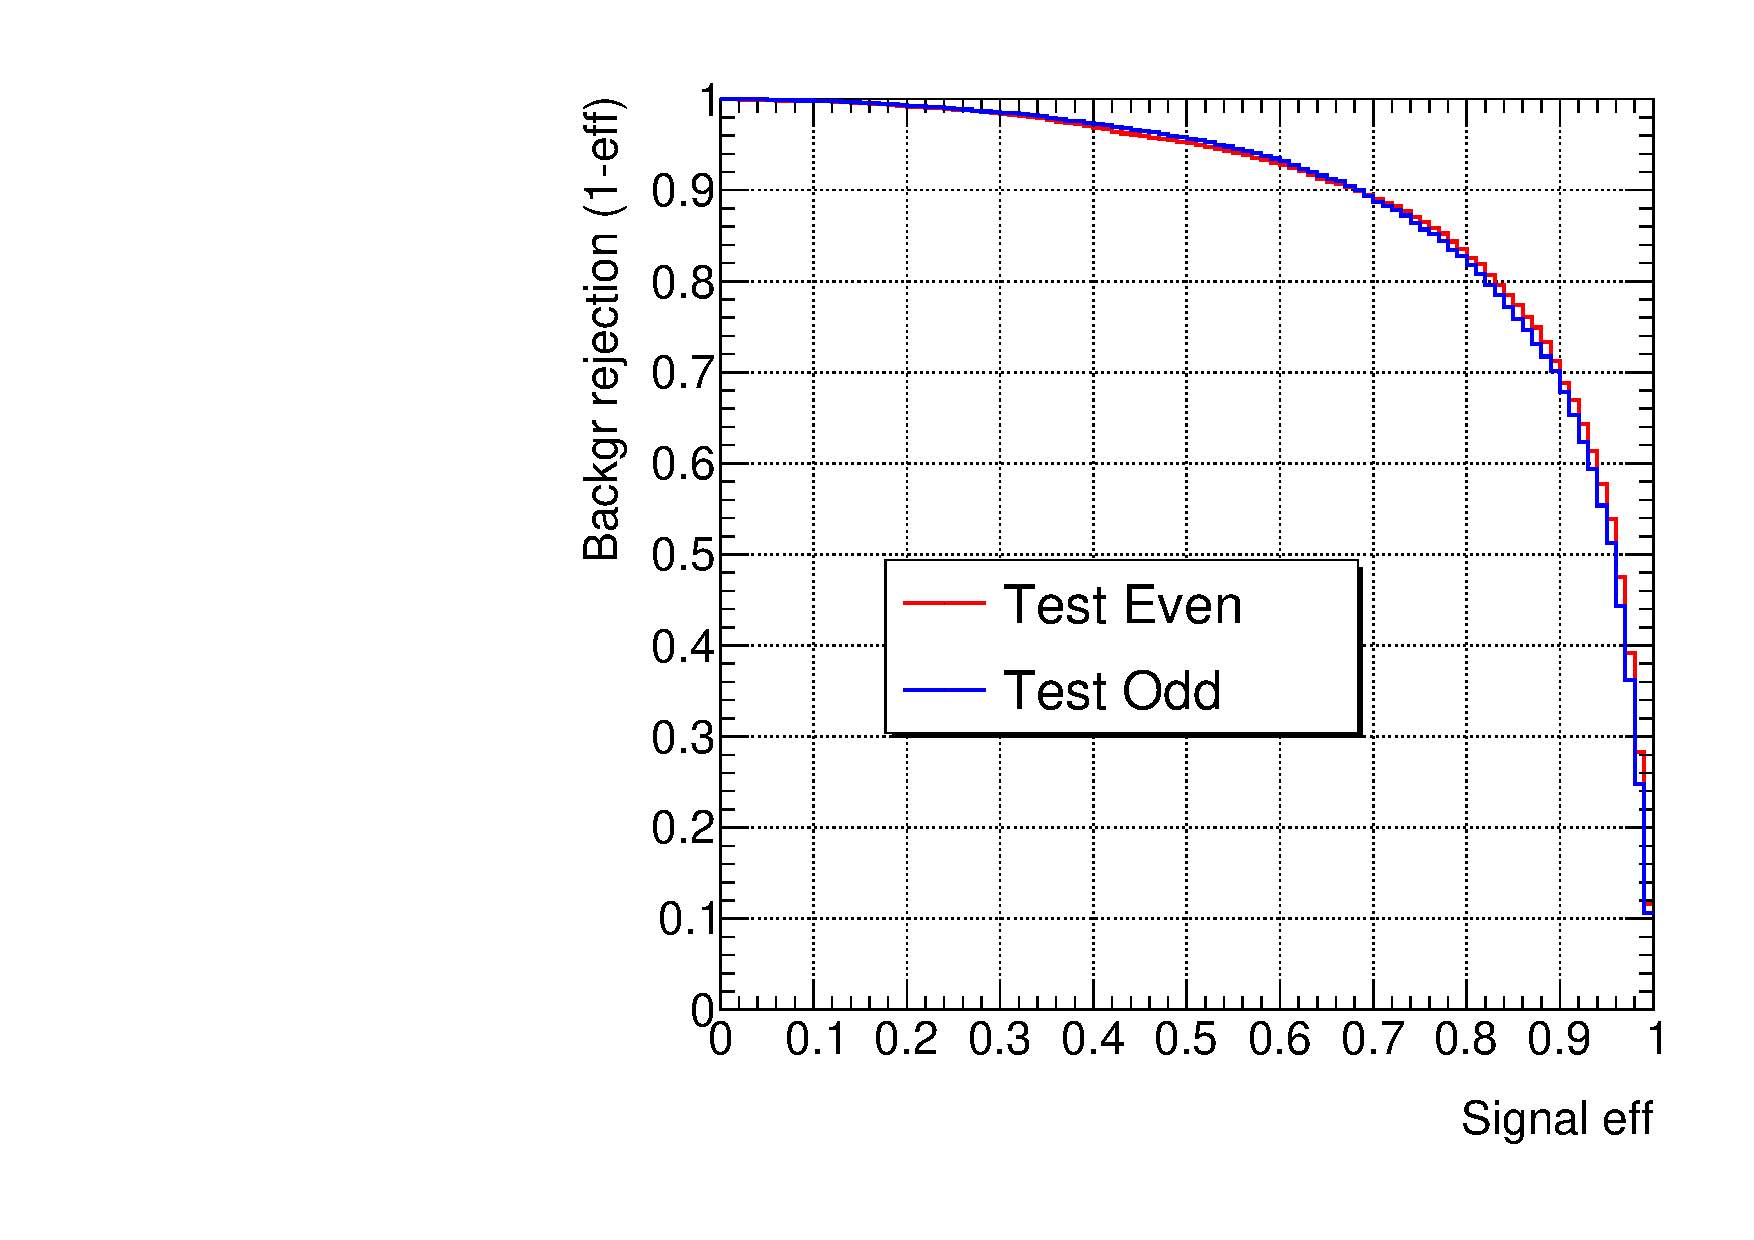
\includegraphics[width=0.33\textwidth]{\FCNCFigures/xTFW/BDT/roc_reg2mtau1b3jos.pdf}
\put(-70, 70){\textbf{(b3)}}\\
\caption{ The BDT output distributions for the background and TT signal (a1, b1), background and ST signal (a2, b2) and ROC curves (a3, b3) in the STH $\thadhad$ (a1-3), TTH $\thadhad$ (b1-3). }% The Kolmogorov Test values for the training and testing BDT distributions are also indicated.
\label{fig:overtrain_hadhad}
\end{figure}
\begin{figure}[htb]
\centering
\includegraphics[page=4,width=0.33\textwidth]{\FCNCFigures/tthML/showFake/faketau/postfit/NOMINAL/reg1l1tau1b2j_os_vetobtagwp70_highmet/BDTG_test.pdf}
\put(-30, 80){\textbf{(a1)}}
\includegraphics[page=5,width=0.33\textwidth]{\FCNCFigures/tthML/showFake/faketau/postfit/NOMINAL/reg1l1tau1b2j_os_vetobtagwp70_highmet/BDTG_test.pdf}
\put(-30, 80){\textbf{(a2)}}
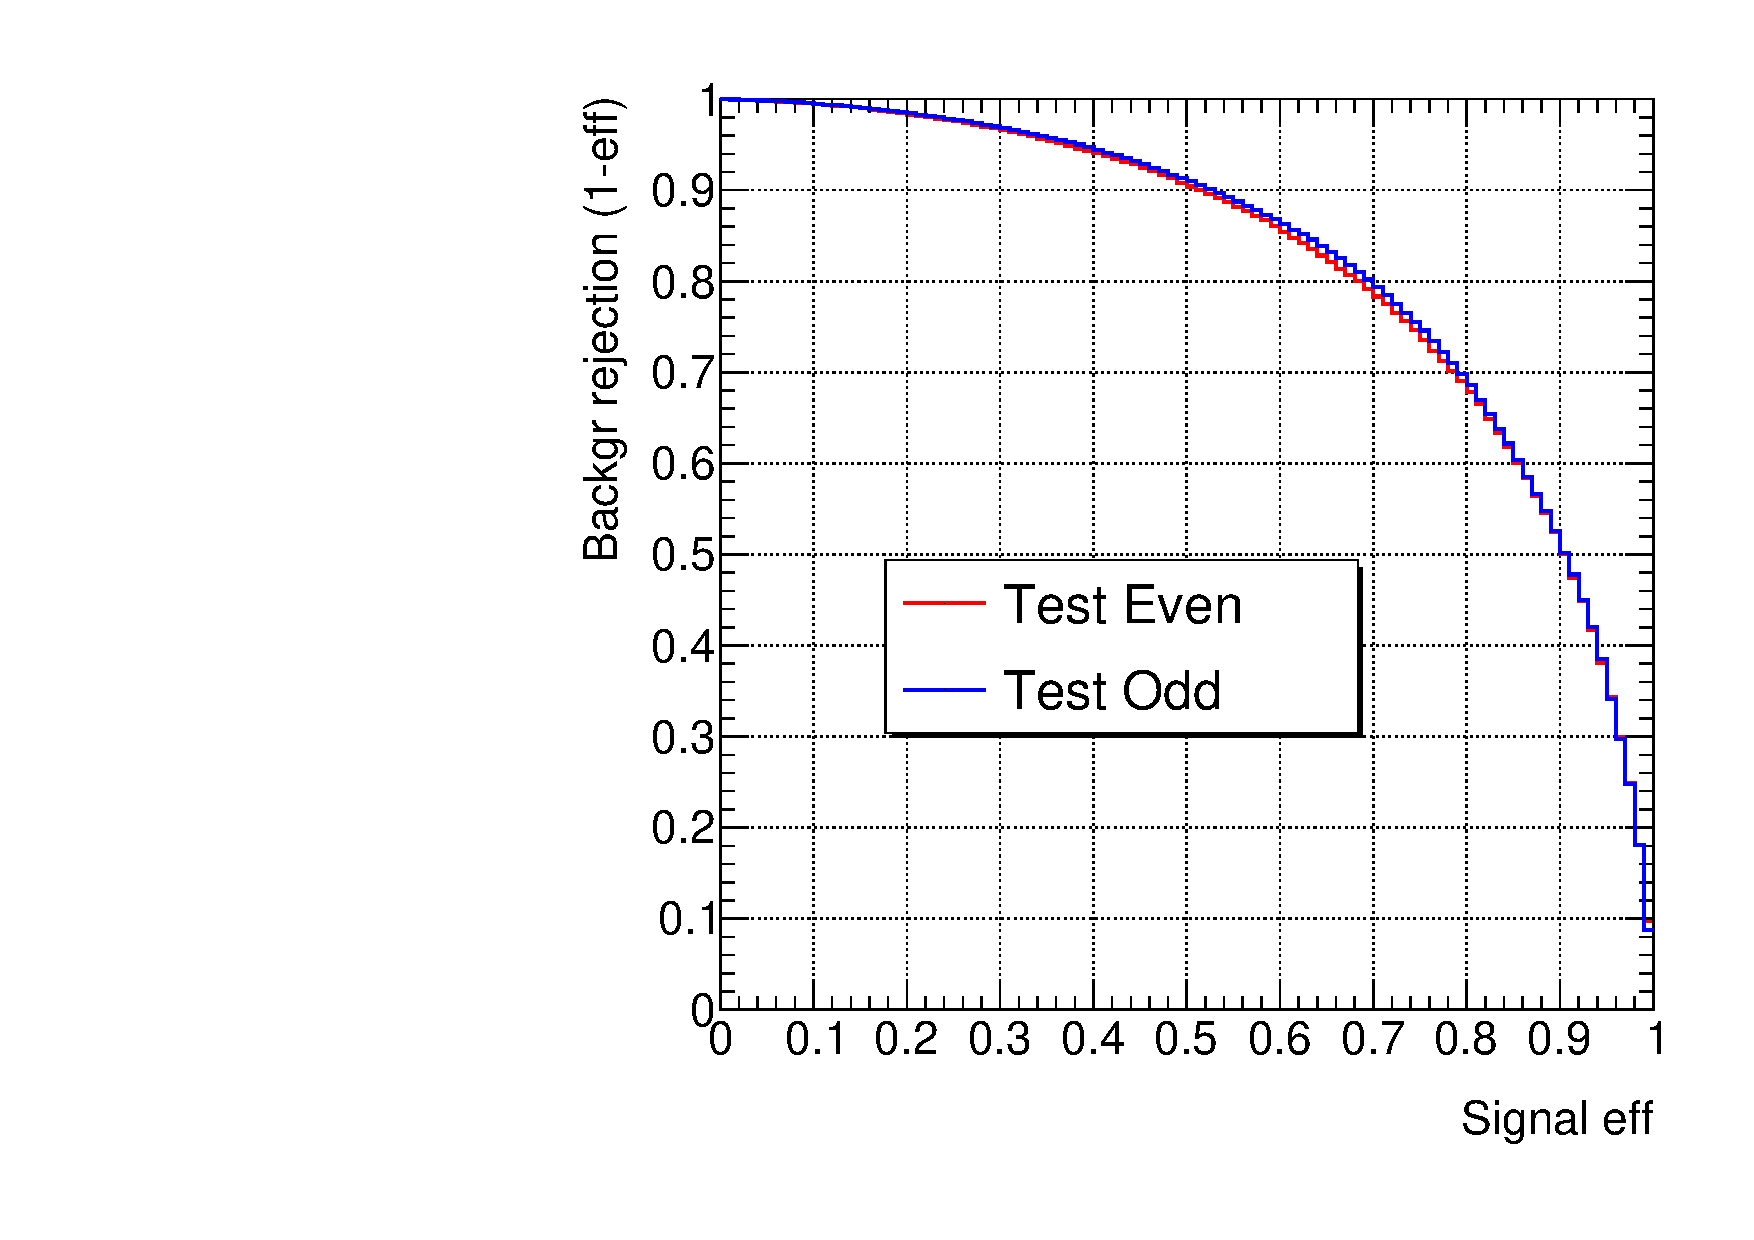
\includegraphics[width=0.33\textwidth]{\FCNCFigures/tthML/BDT/roc_reg1l1tau1b2j_os.pdf}
\put(-70, 85){\textbf{(a3)}}\\
\includegraphics[page=4,width=0.33\textwidth]{\FCNCFigures/tthML/showFake/faketau/postfit/NOMINAL/reg1l1tau1b3j_os_vetobtagwp70_highmet/BDTG_test.pdf}
\put(-30, 80){\textbf{(b1)}}
\includegraphics[page=5,width=0.33\textwidth]{\FCNCFigures/tthML/showFake/faketau/postfit/NOMINAL/reg1l1tau1b3j_os_vetobtagwp70_highmet/BDTG_test.pdf}
\put(-30, 80){\textbf{(b2)}}
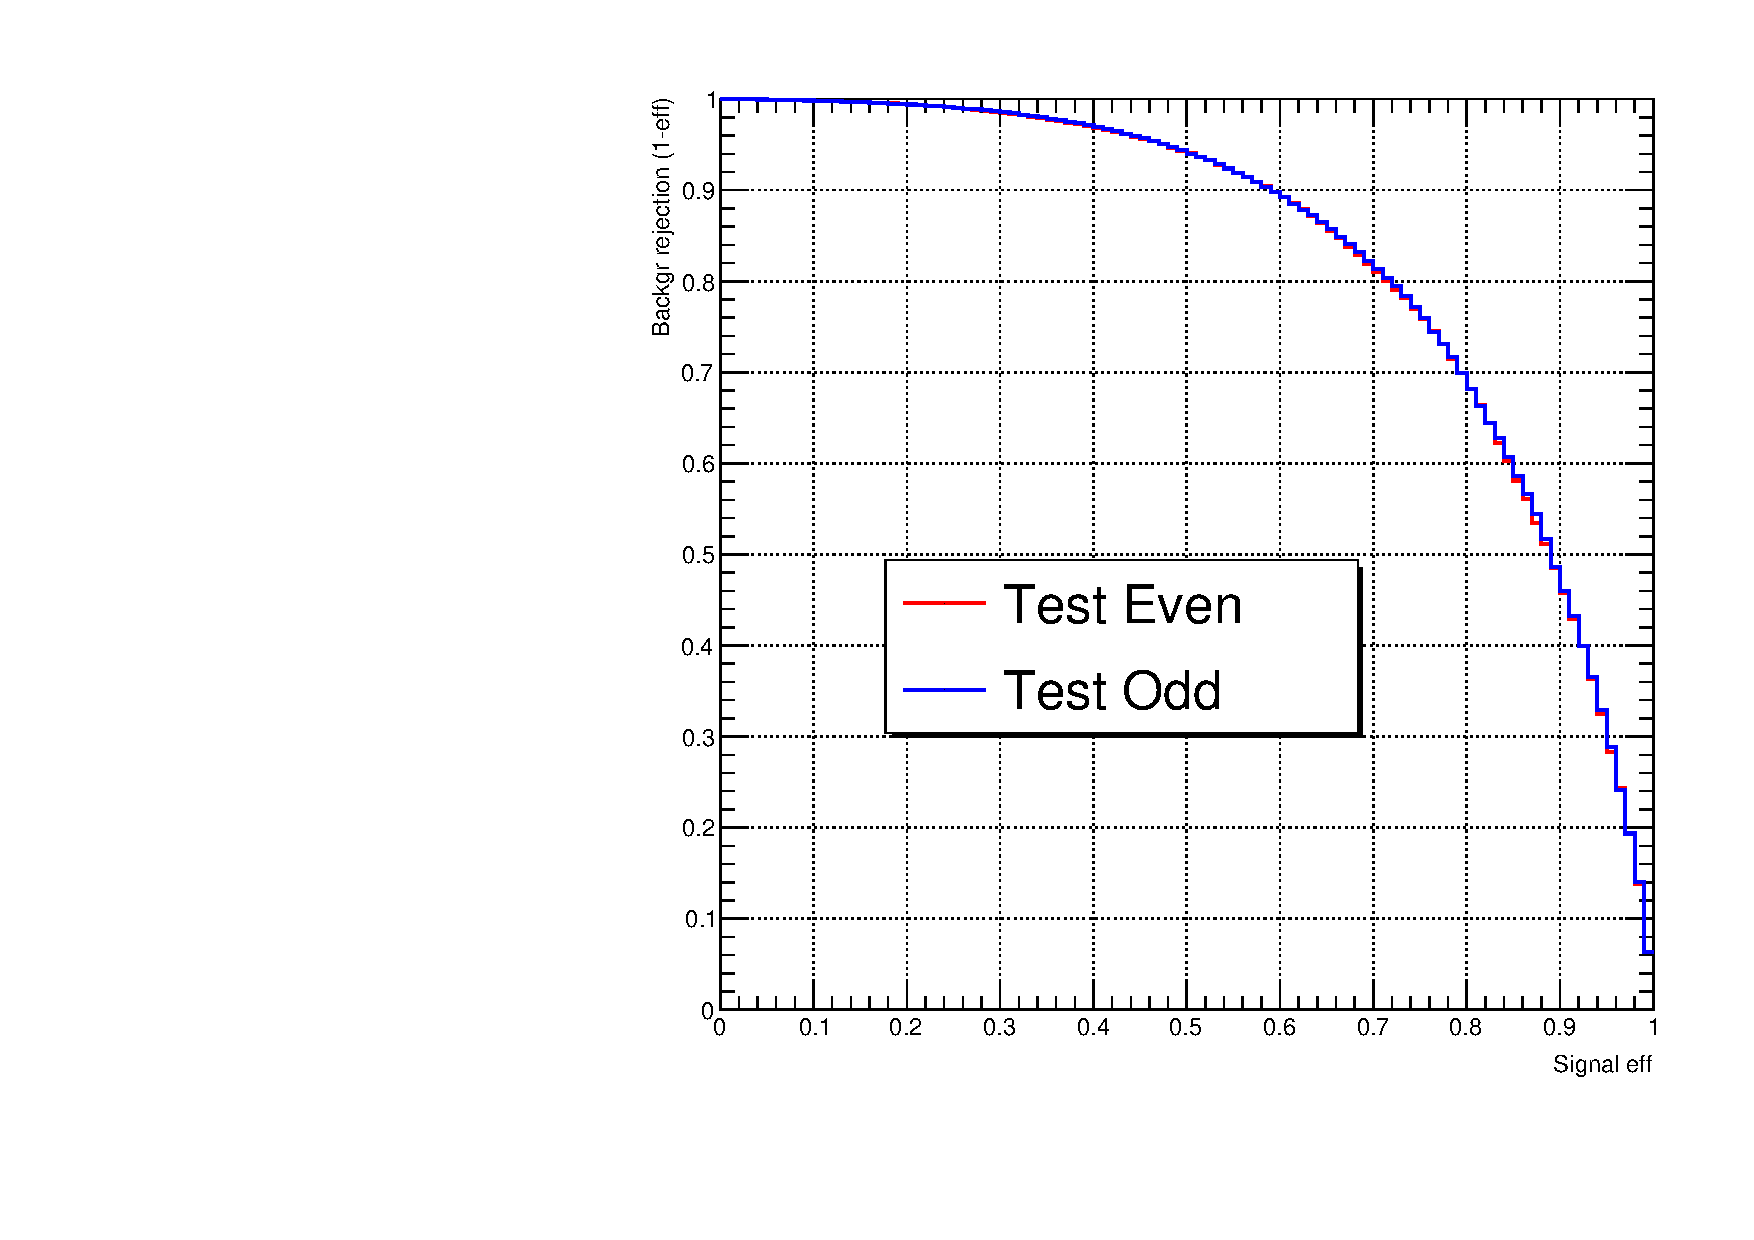
\includegraphics[width=0.33\textwidth]{\FCNCFigures/tthML/BDT/roc_reg1l1tau1b3j_os.pdf}
\put(-70, 85){\textbf{(b3)}}\\
\caption{ The BDT output distributions for the background and TT signal (a1, b1), background and ST signal (a2, b2) and ROC curves (a3, b3) in the STH $\tlhad$ (a1-3), TTH $\tlhad$ (b1-3). }% The Kolmogorov Test values for the training and testing BDT distributions are also indicated.
\label{fig:overtrain_lephad}
\end{figure}
\begin{figure}[htb]
\centering
\includegraphics[page=4,width=0.33\textwidth]{\FCNCFigures/tthML/showFake/faketau/postfit/NOMINAL/reg1l2tau1bnj_os/BDTG_test.pdf}
\put(-30, 80){\textbf{(a1)}}
\includegraphics[page=5,width=0.33\textwidth]{\FCNCFigures/tthML/showFake/faketau/postfit/NOMINAL/reg1l2tau1bnj_os/BDTG_test.pdf}
\put(-30, 80){\textbf{(a2)}}
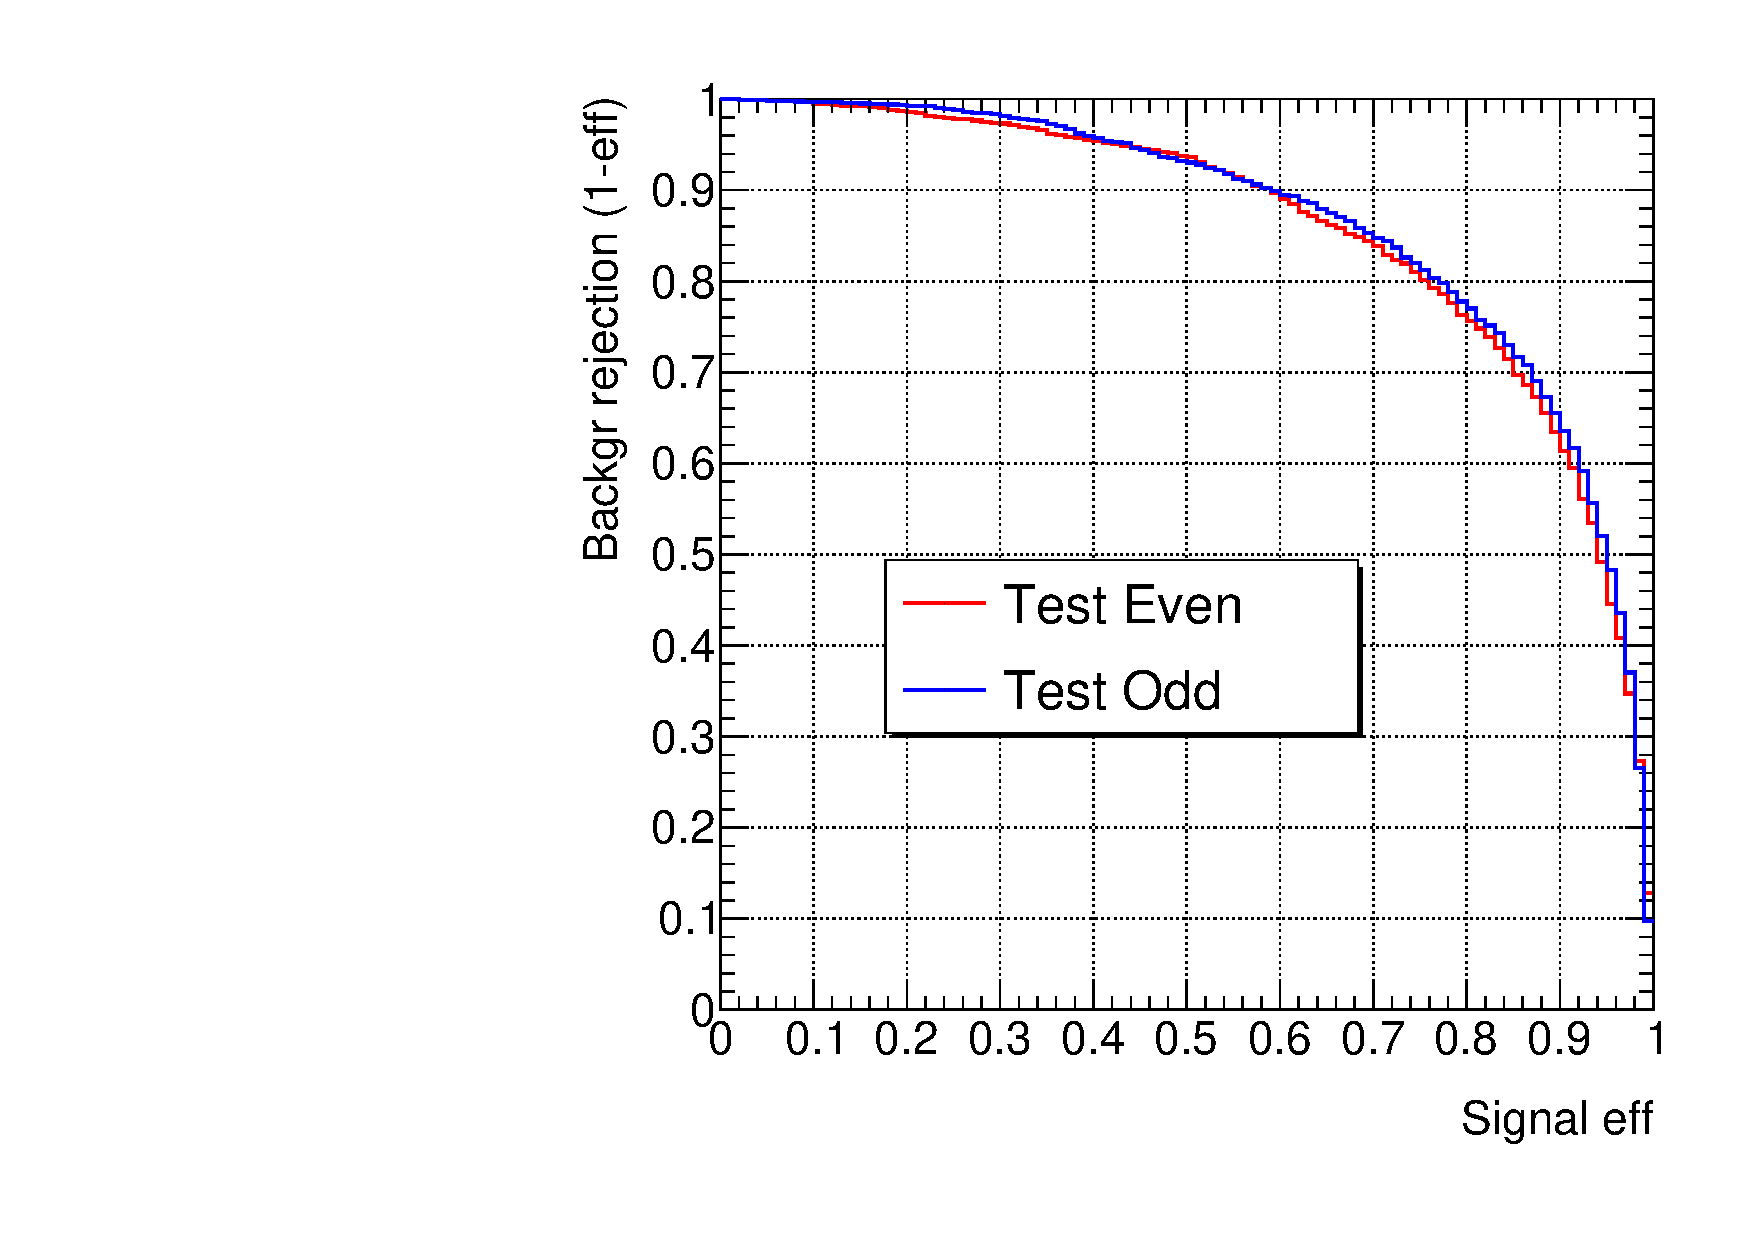
\includegraphics[width=0.33\textwidth]{\FCNCFigures/tthML/BDT/roc_reg1l2tau1bnj_os.pdf}
\put(-70, 85){\textbf{(a3)}}\\

\includegraphics[page=4,width=0.33\textwidth]{\FCNCFigures/tthML/showFake/faketau/postfit/NOMINAL/reg1l1tau1b1j_ss_vetobtagwp70_highmet/BDTG_test.pdf}
\put(-30, 80){\textbf{(b1)}}
\includegraphics[page=5,width=0.33\textwidth]{\FCNCFigures/tthML/showFake/faketau/postfit/NOMINAL/reg1l1tau1b1j_ss_vetobtagwp70_highmet/BDTG_test.pdf}
\put(-30, 80){\textbf{(b2)}}
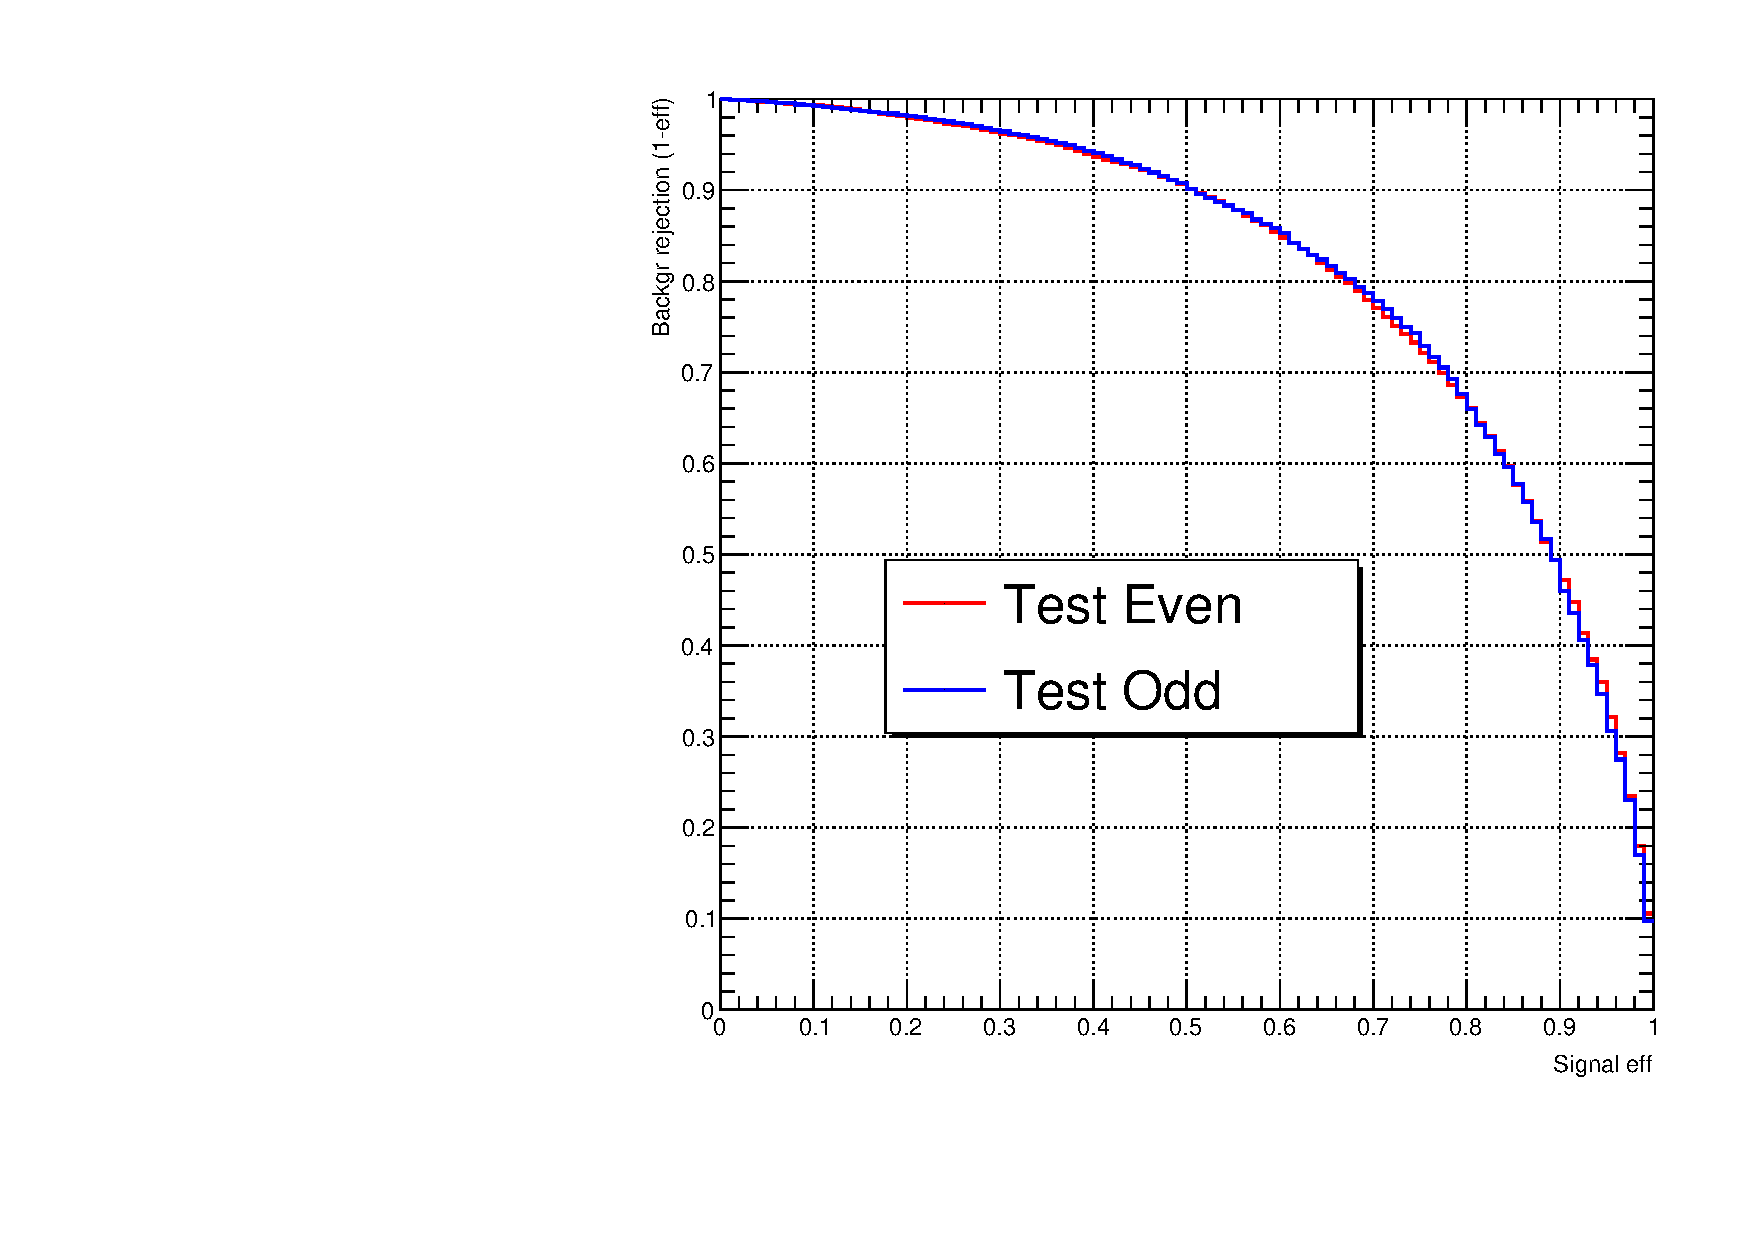
\includegraphics[width=0.33\textwidth]{\FCNCFigures/tthML/BDT/roc_reg1l1tau1b1j_ss.pdf}
\put(-70, 85){\textbf{(b3)}}\\

\includegraphics[page=4,width=0.33\textwidth]{\FCNCFigures/tthML/showFake/faketau/postfit/NOMINAL/reg1l1tau1b2j_ss_vetobtagwp70_highmet/BDTG_test.pdf}
\put(-30, 80){\textbf{(c1)}}
\includegraphics[page=5,width=0.33\textwidth]{\FCNCFigures/tthML/showFake/faketau/postfit/NOMINAL/reg1l1tau1b2j_ss_vetobtagwp70_highmet/BDTG_test.pdf}
\put(-30, 80){\textbf{(c2)}}
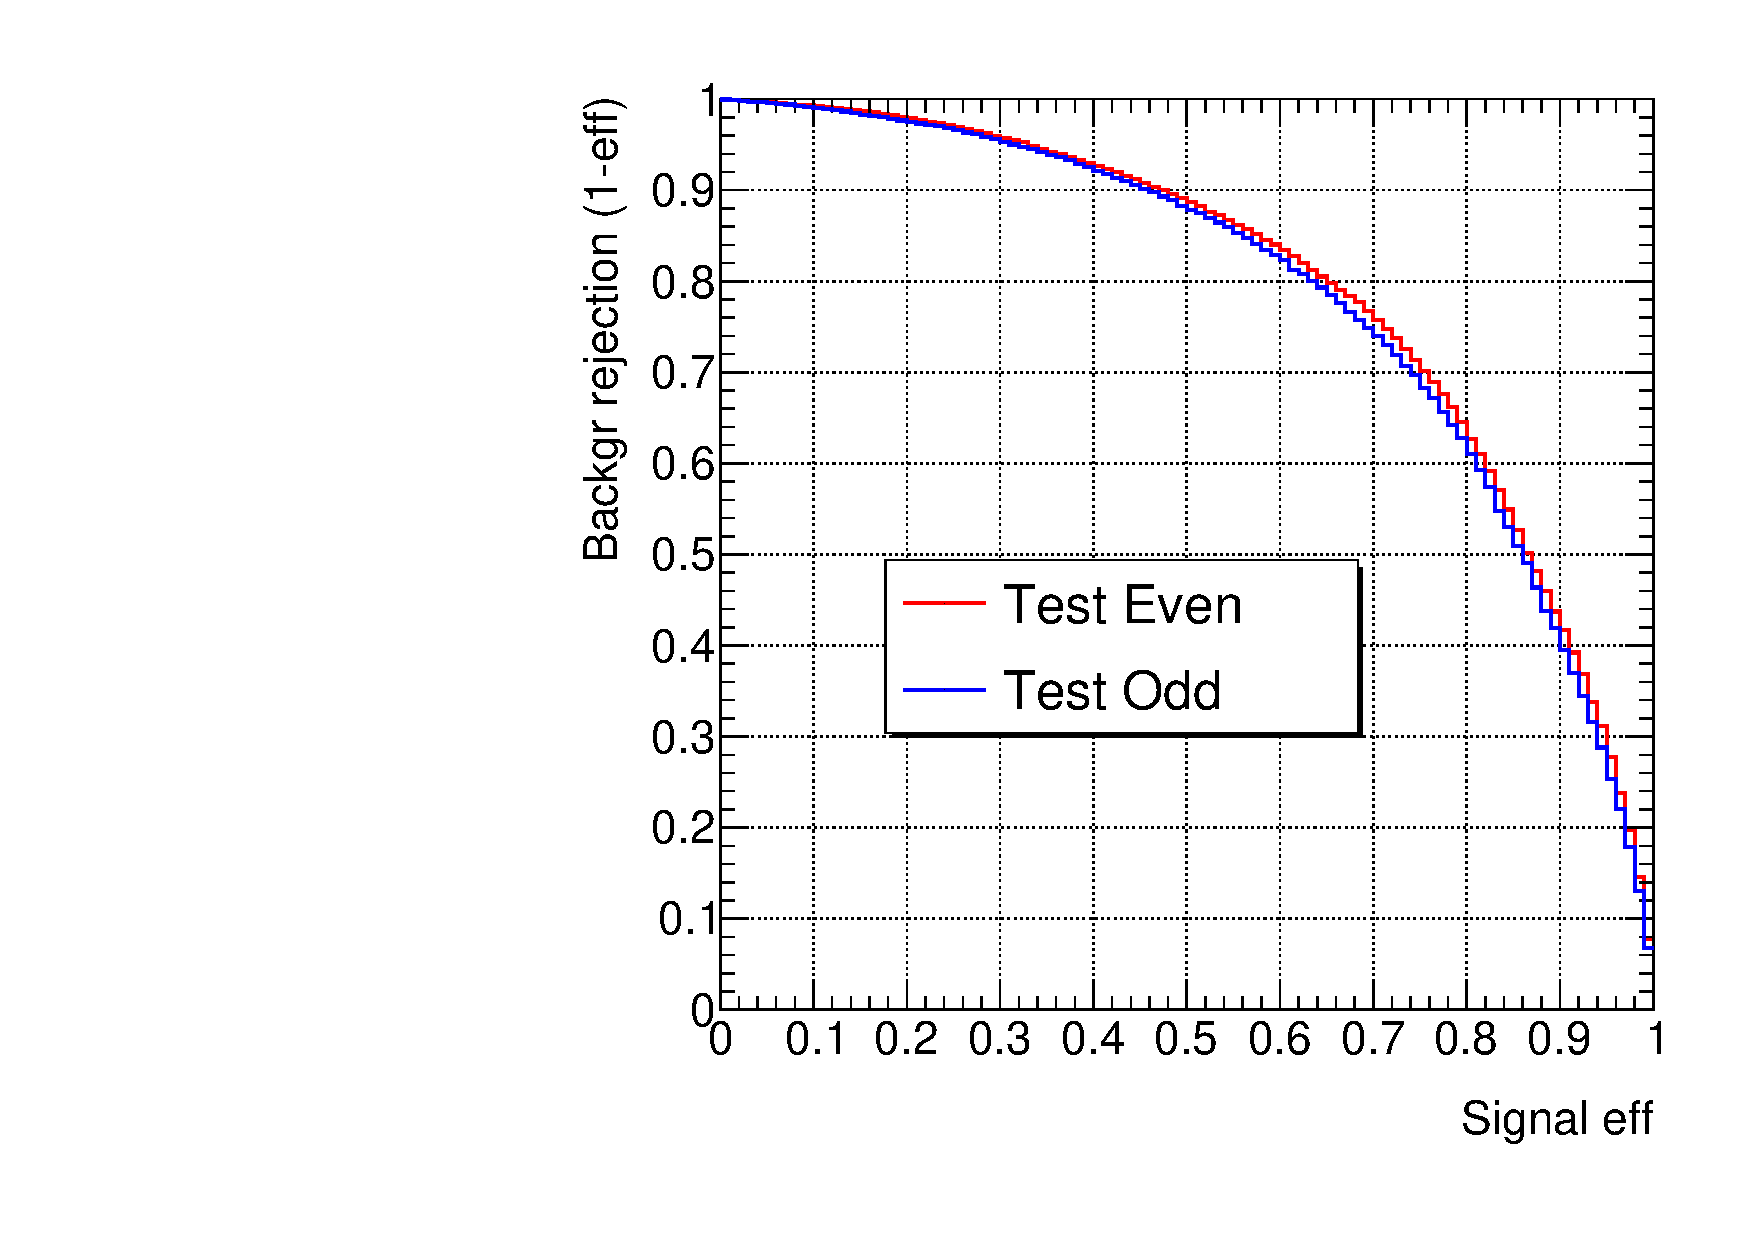
\includegraphics[width=0.33\textwidth]{\FCNCFigures/tthML/BDT/roc_reg1l1tau1b2j_ss.pdf}
\put(-70, 85){\textbf{(c3)}}\\

\caption{ The BDT output distributions for the background and TT signal (a1, b1, c1), background and ST signal (a2, b2, c2) and ROC curves (a3, b3, c3) in the $l\thadhad$ (a1-3), $\tauhad$ 1j (b1-3), $\tauhad$ 2j (c1-3) channels. }% The Kolmogorov Test values for the training and testing BDT distributions are also indicated.
\label{fig:overtrain_lhadhad}
\end{figure}
